\chapter {Fase II: Diseño}
\label{cap:Fase II.Diseño}

Medicina y Tecnología han caminado juntas desde el principio de los tiempos: desde el instrumental quirúrgico y su evolución a lo largo de los siglos, pasando por el fonendoscopio, las prótesis, el electrocardiograma, las radiografías o la resonancia magnética. Son muchos los avances tecnológicos que han facilitado la labor de los médicos a la hora de emitir diagnósticos y aplicar tratamientos.

\section{Prototipado de la GUI}
\subsection{Ventana de Inicio}
\begin{figure}[htb]
	\centering
	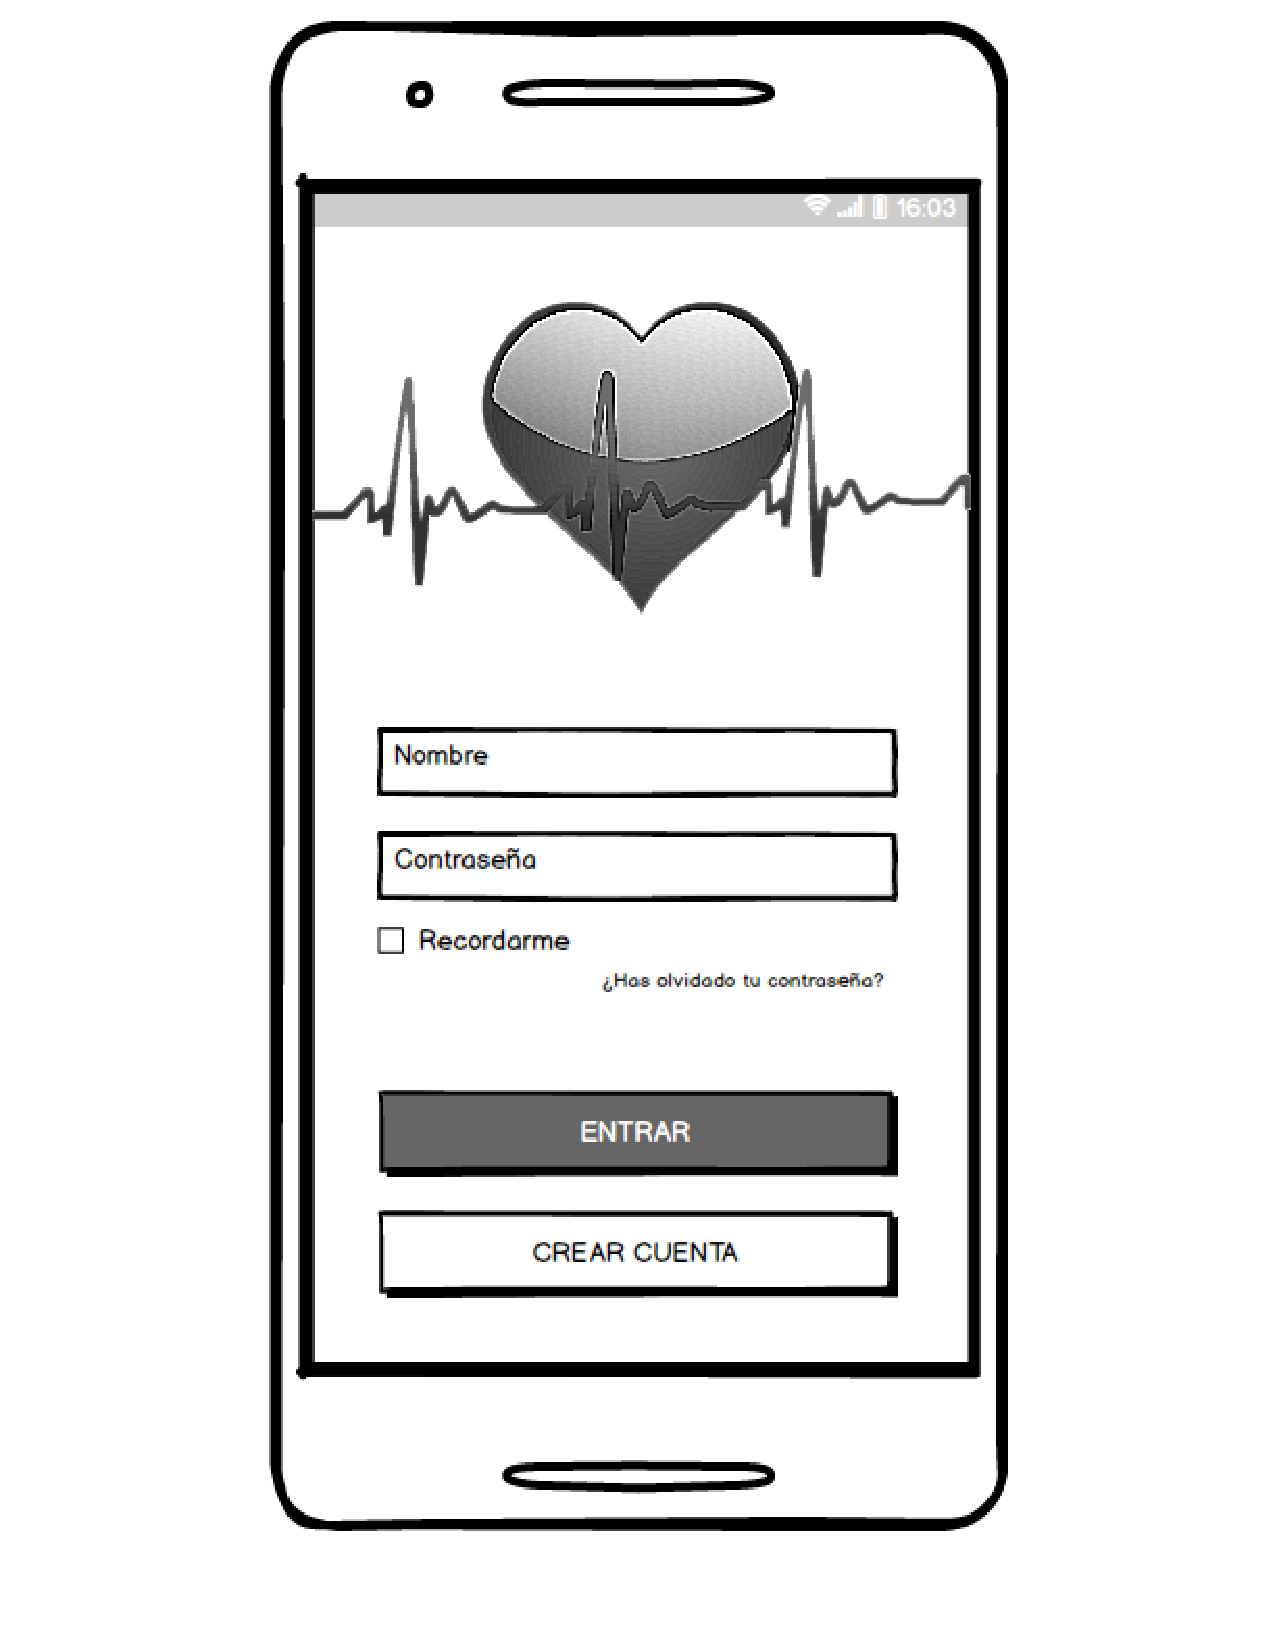
\includegraphics[width=0.4\textwidth]{GSI-1} 
	\caption[Ventana de Inicio]{Ventana de inicio}
	
	\label{fig:defInicio}
\end{figure}


\subsection{Ventana de Estado}
\begin{figure}[htb]
	\centering
	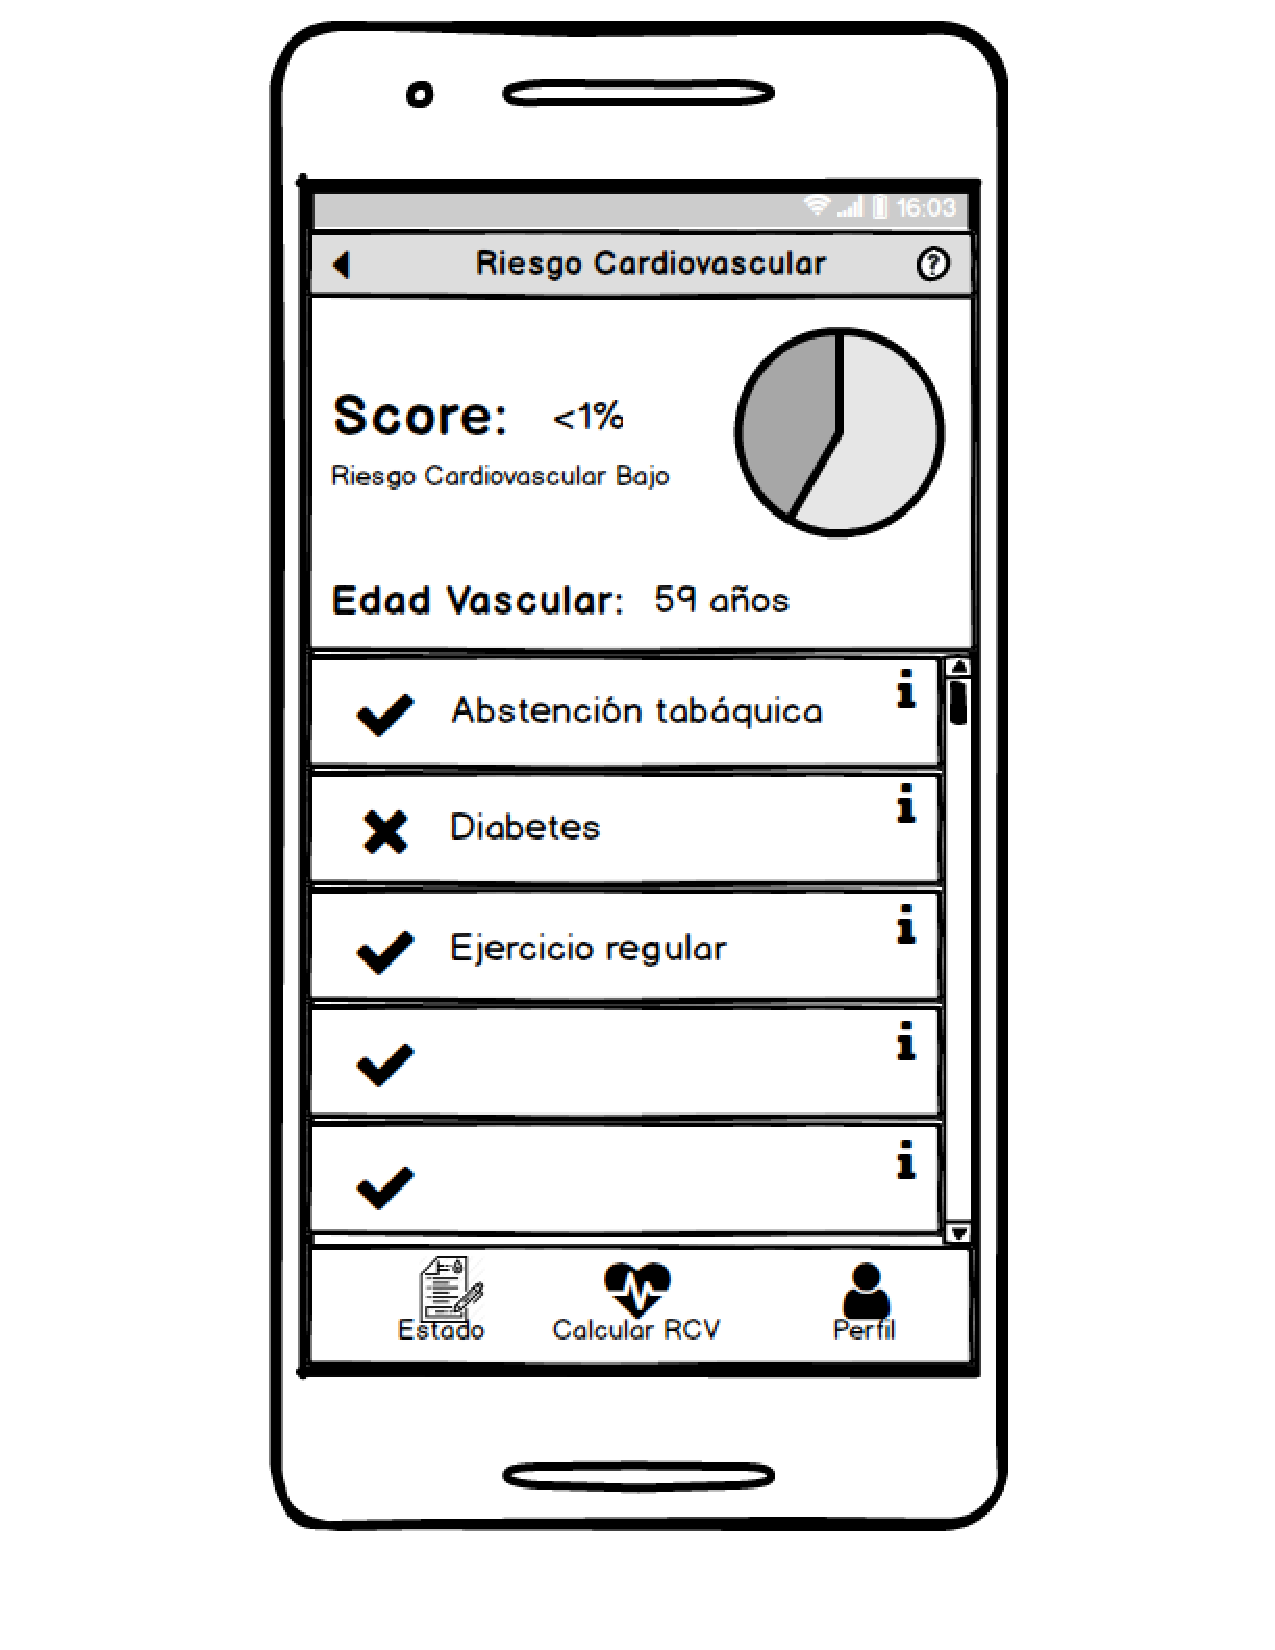
\includegraphics[width=0.4\textwidth]{GSI-2} 
	\caption[Ventana de Estado]{Ventana de Estado}
	
	\label{fig:defEstado}
\end{figure}

\subsection{Ventana de Perfil}
\begin{figure}[htb]
	\centering
	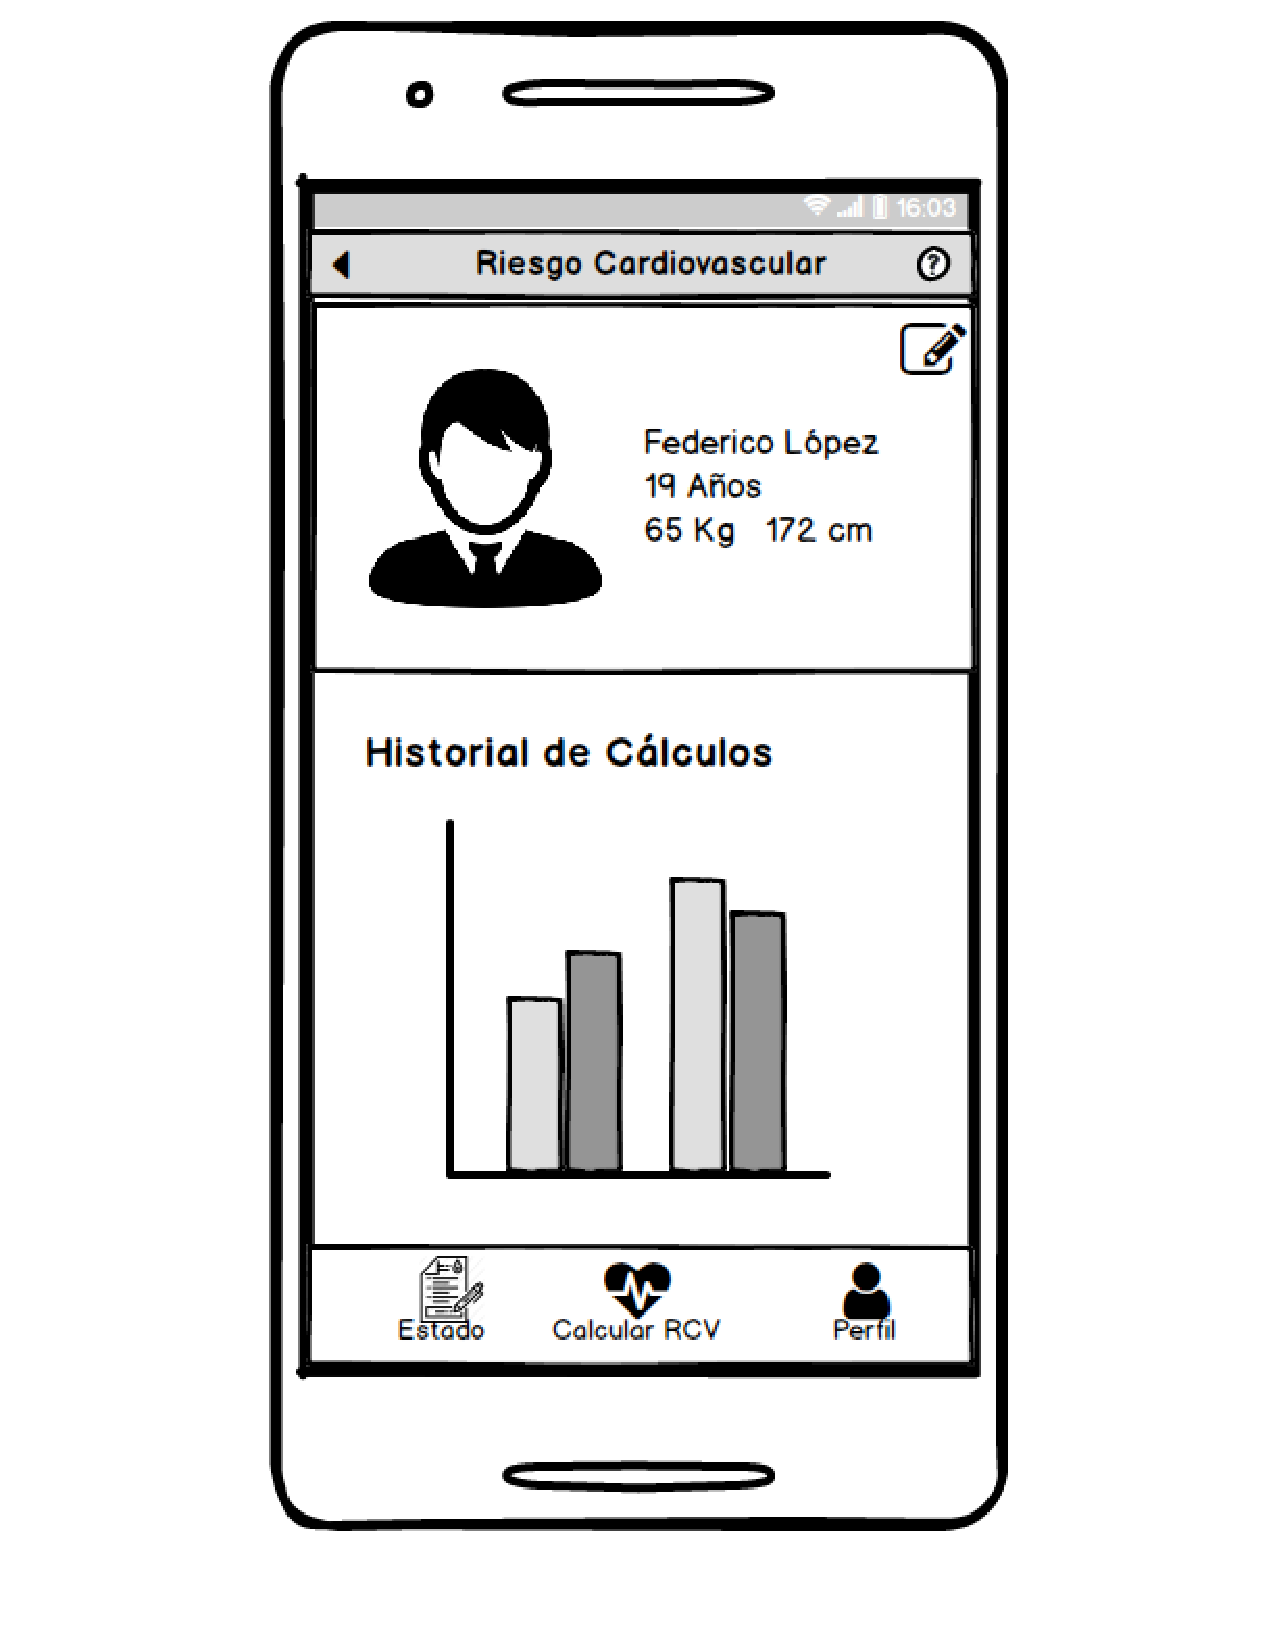
\includegraphics[width=0.4\textwidth]{GSI-3} 
	\caption[Ventana de Perfil]{Ventana de Perfil}
	
	\label{fig:defPerfil}
\end{figure}

\subsection{Ventana de Cálculo del RCV}
\begin{figure}[htb]
	\centering
	\subfigure[]{
		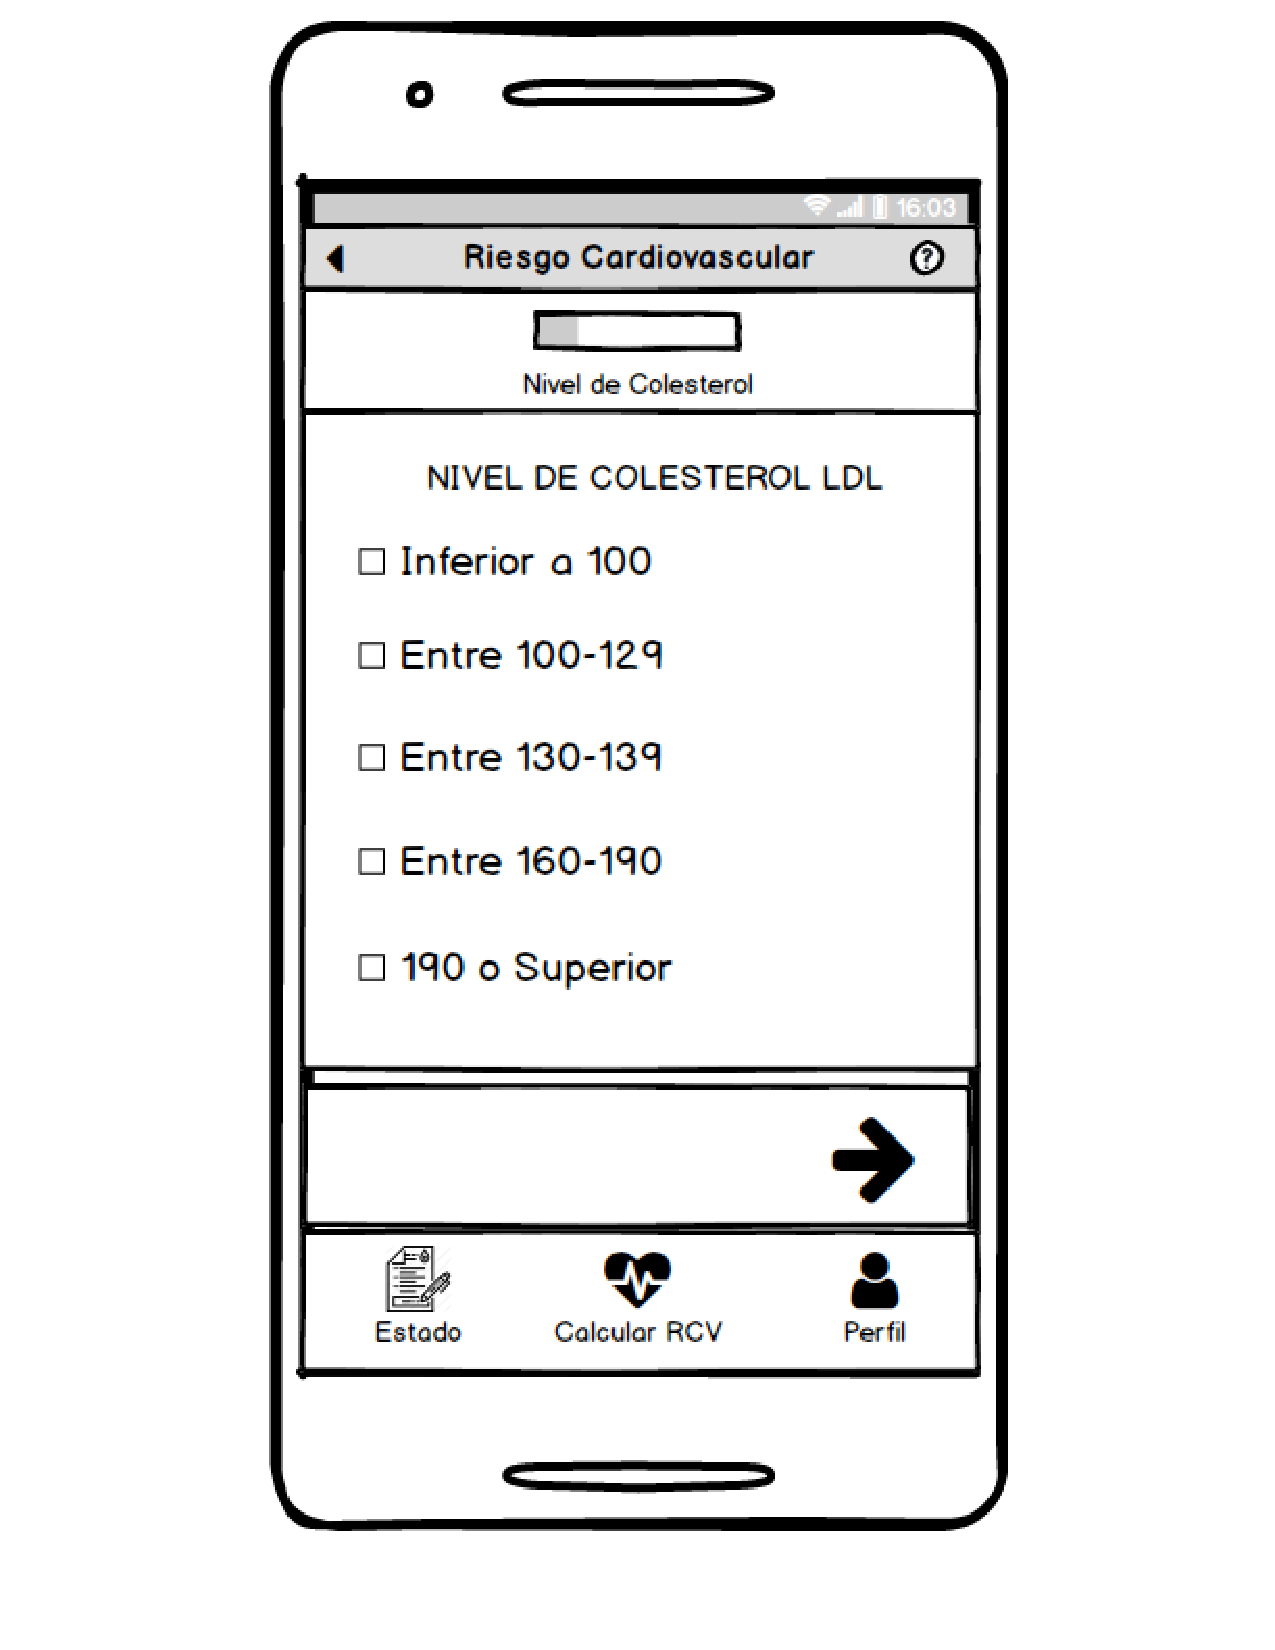
\includegraphics[width=0.3\textwidth]{GSI-4} 
		\label{fig:raCalculo1}
	}
	\subfigure[]{
		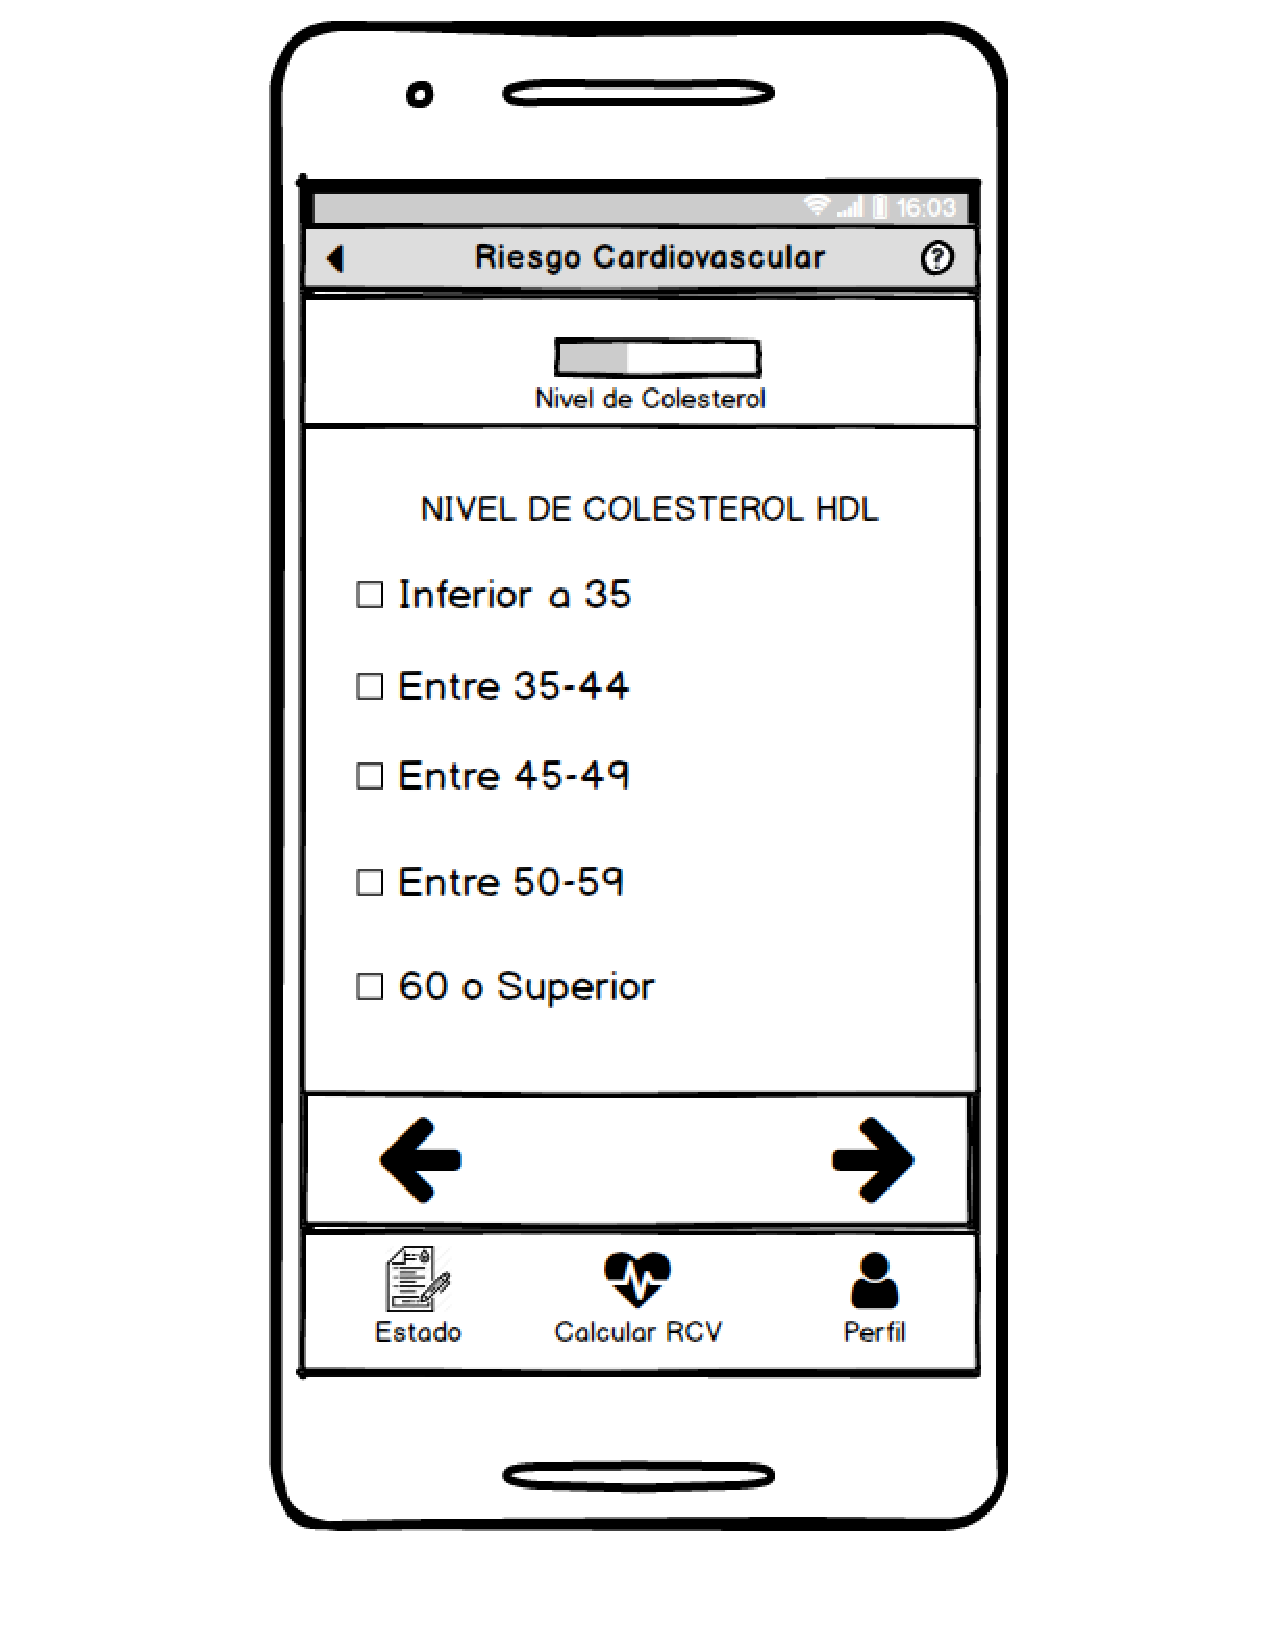
\includegraphics[width=0.3\textwidth]{GSI-5}
		\label{fig:raCalculo2}
	}
		\subfigure[]{
			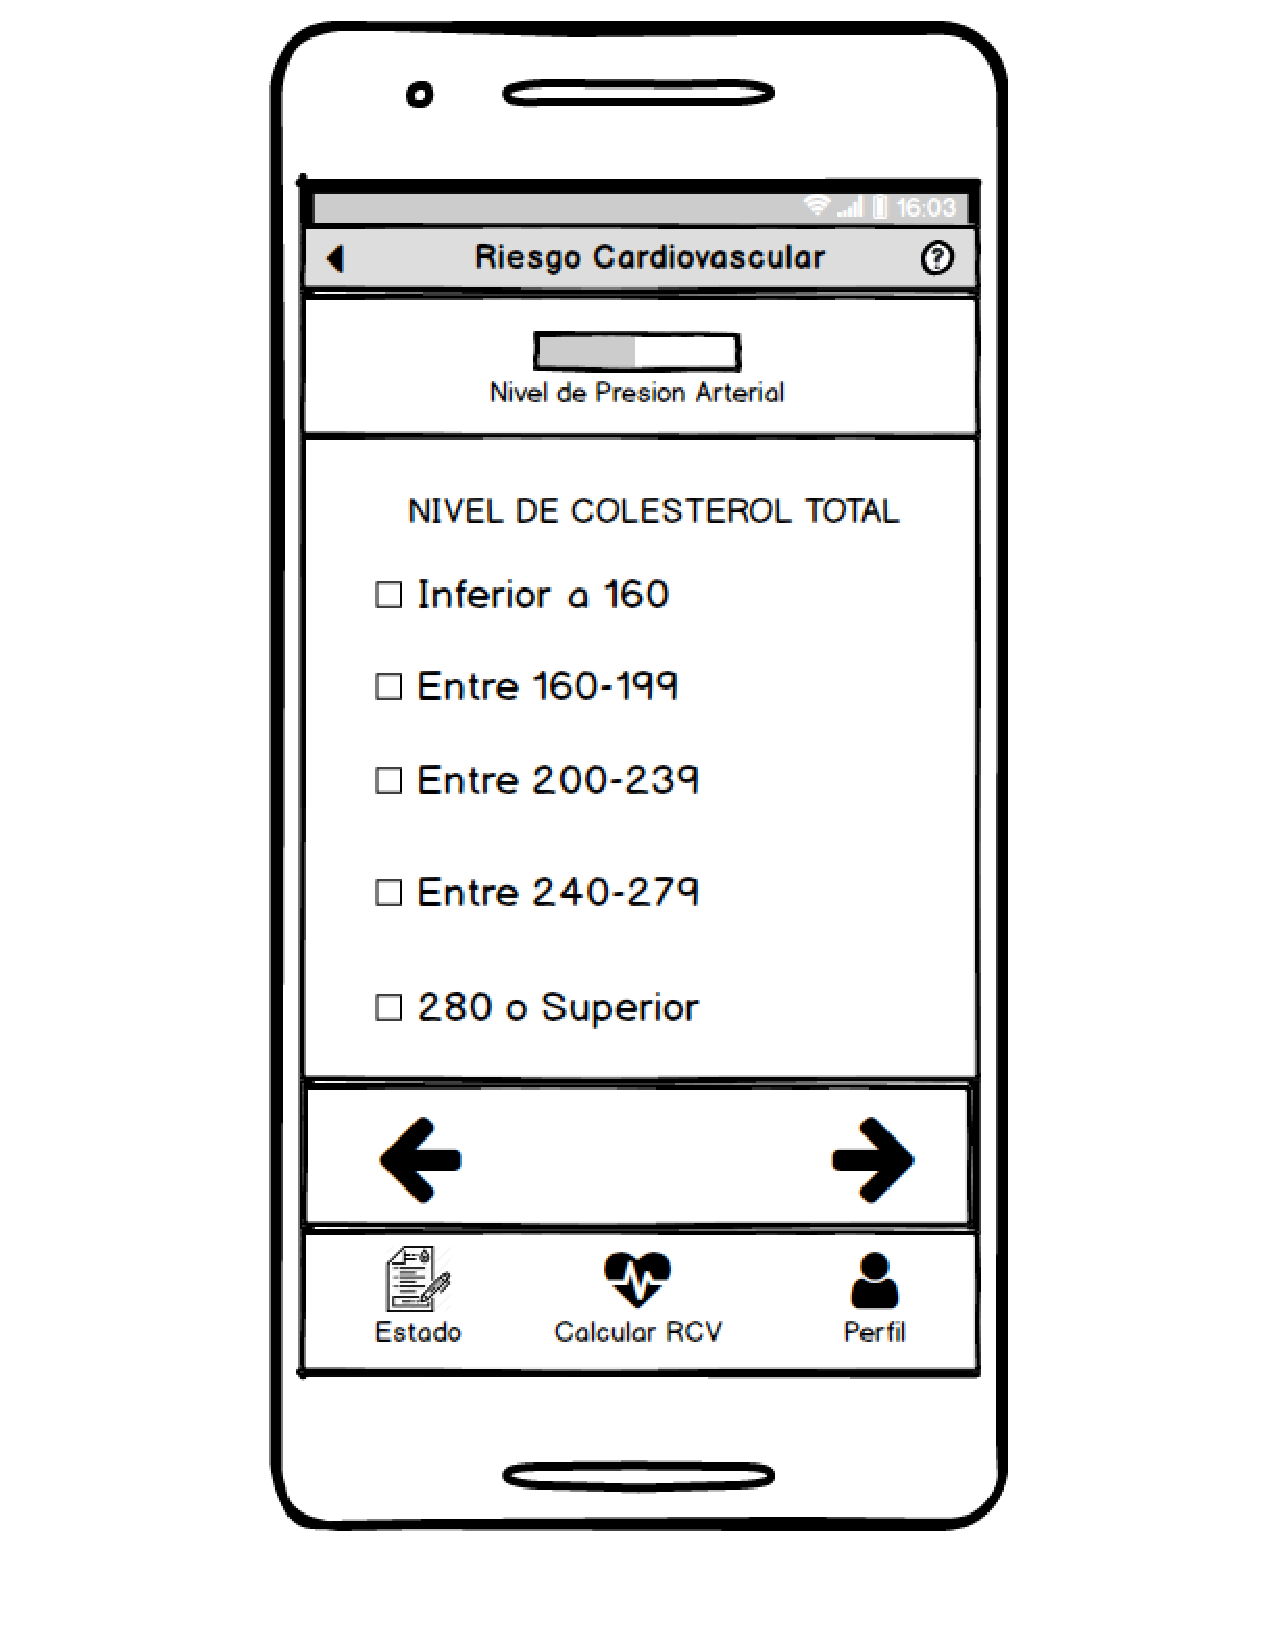
\includegraphics[width=0.3\textwidth]{GSI-6}
			\label{fig:raCalculo3}
		}
		\subfigure[]{
			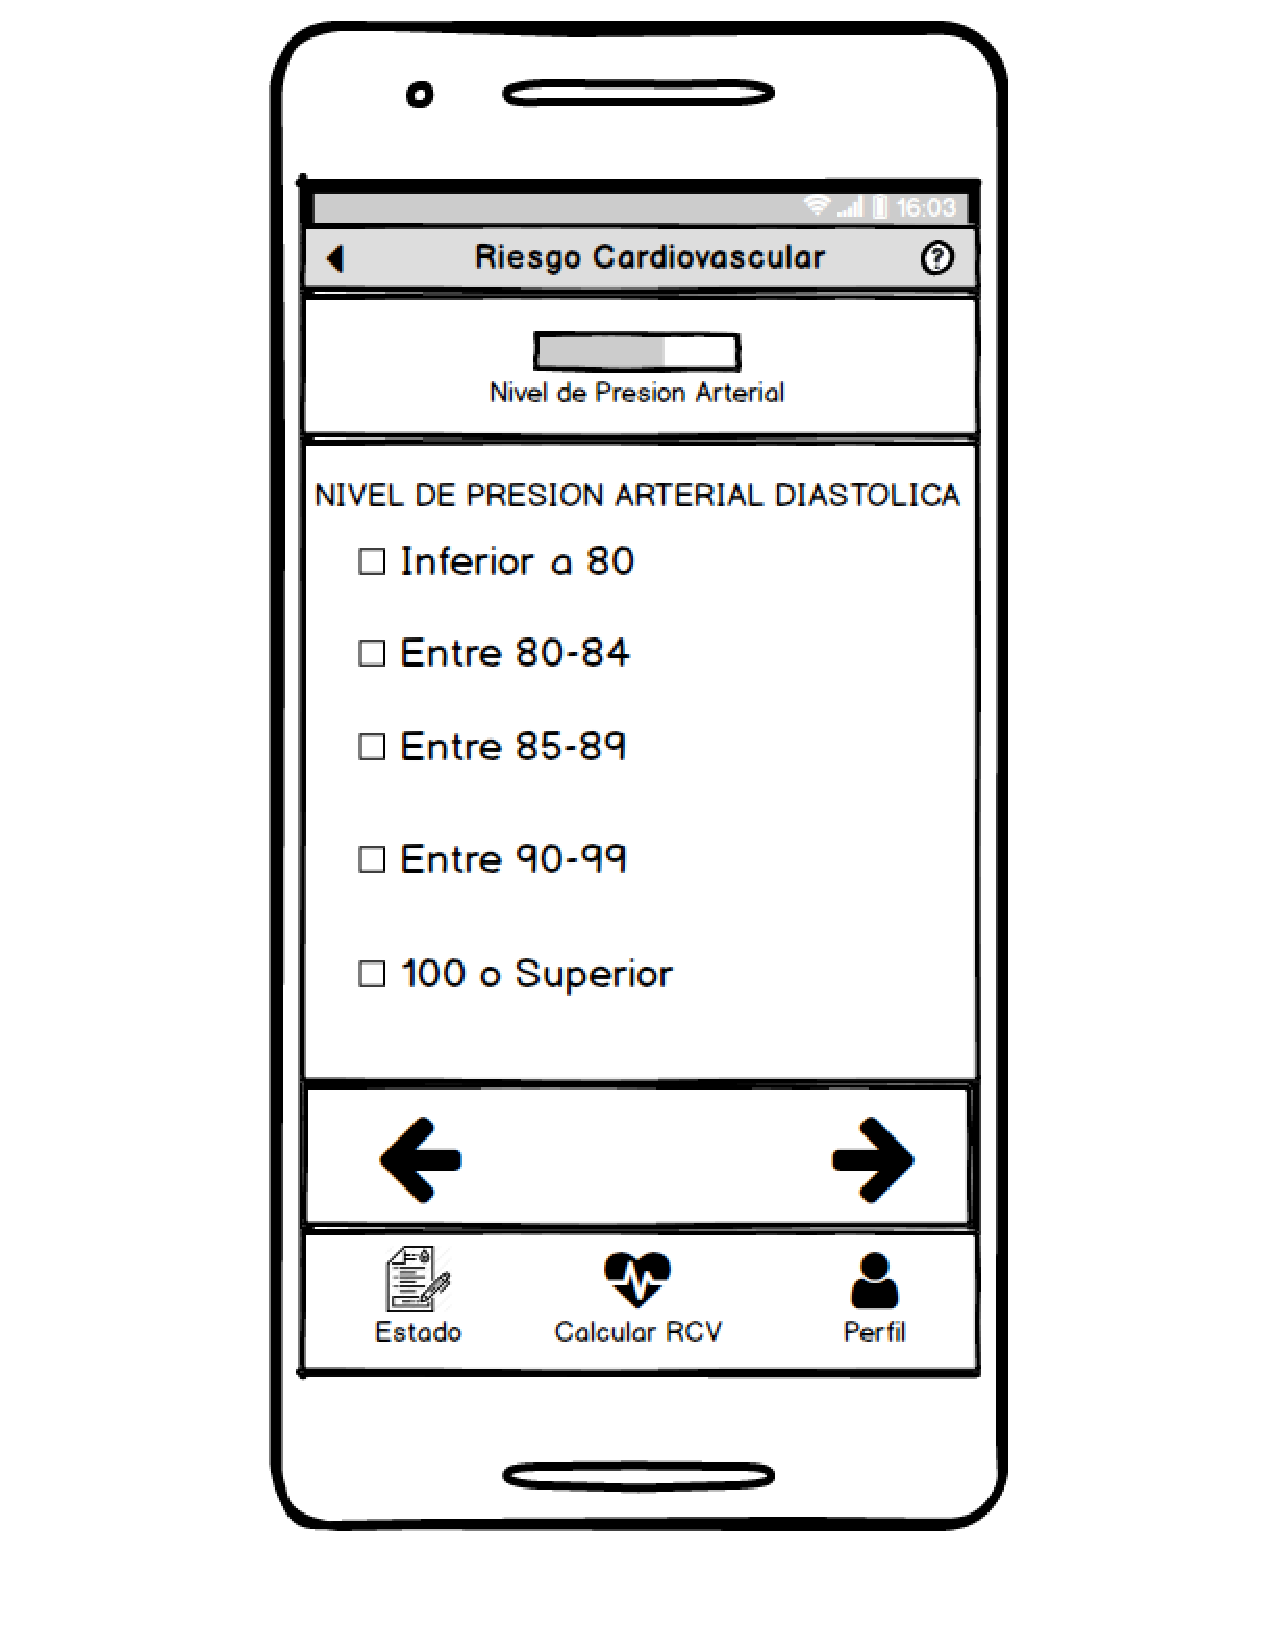
\includegraphics[width=0.3\textwidth]{GSI-7}
			\label{fig:raCalculo4}
		}
		\subfigure[]{
			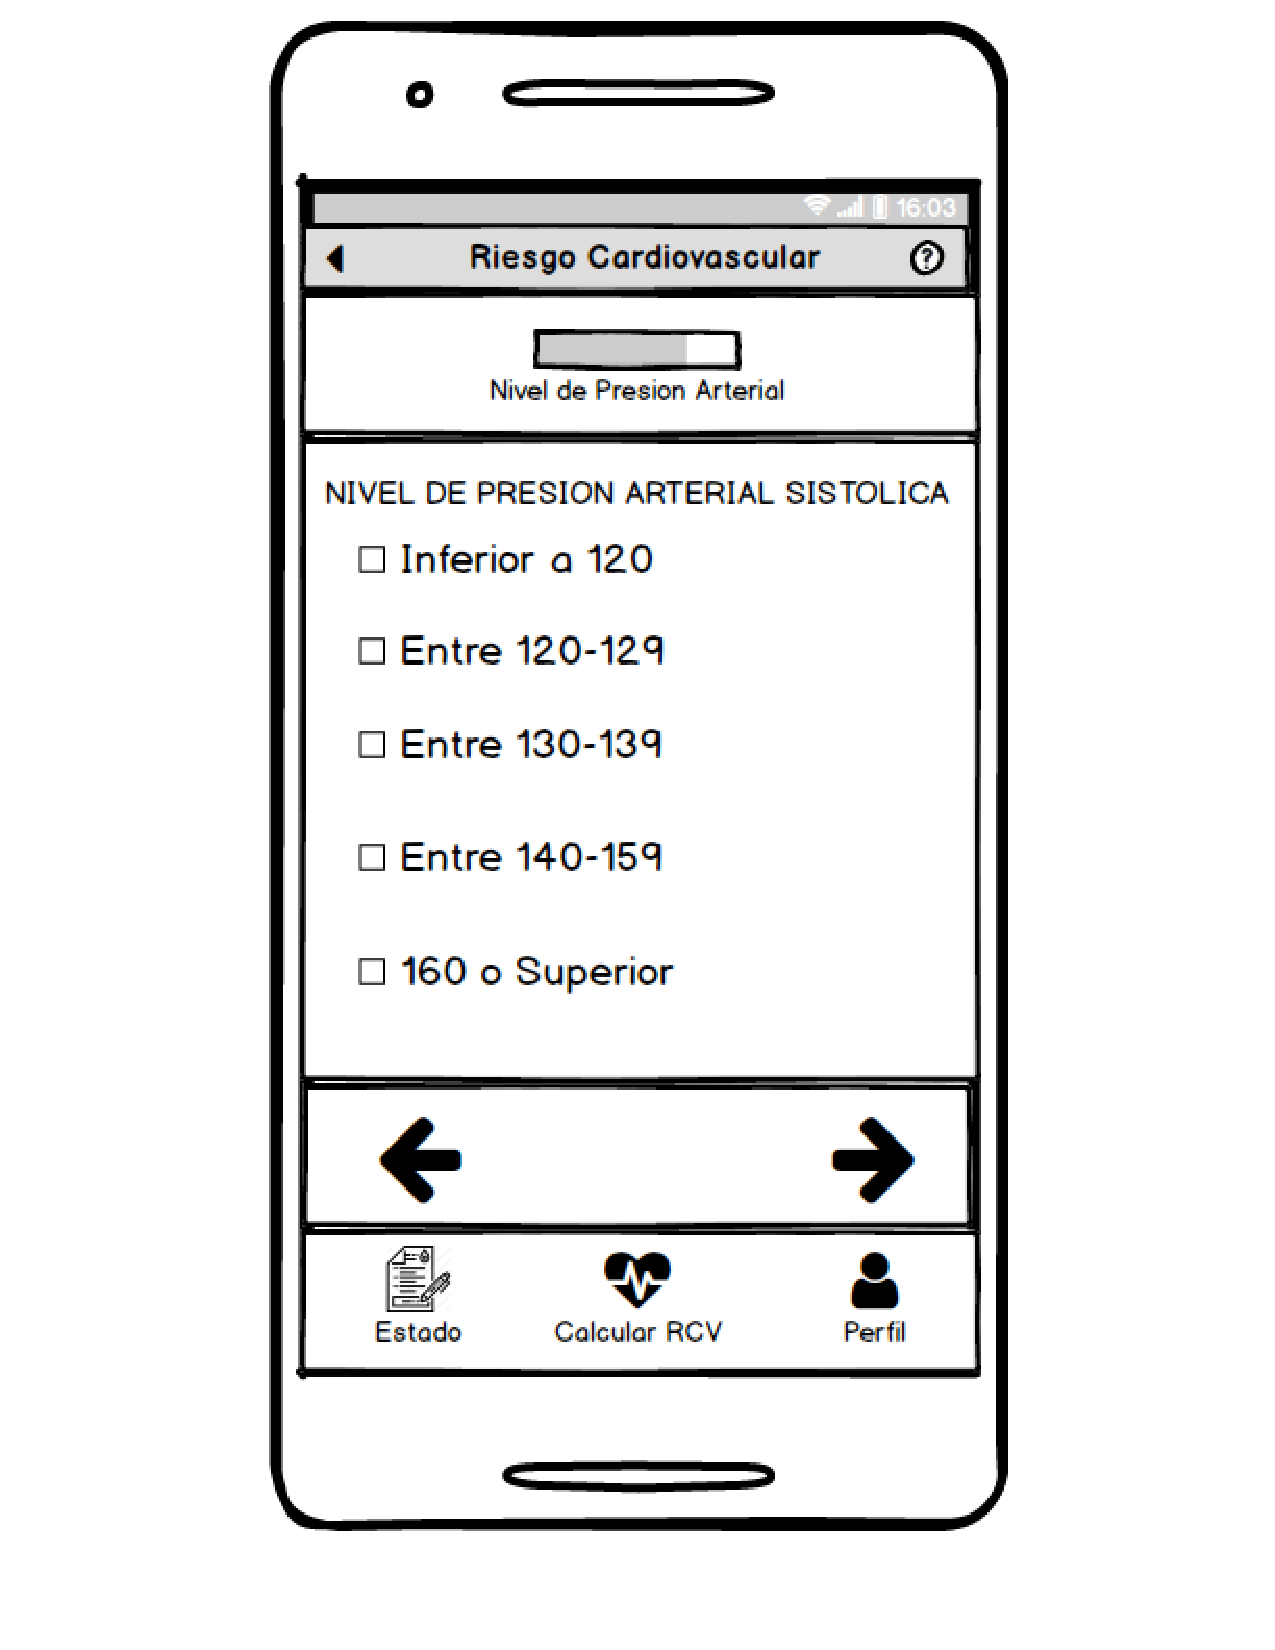
\includegraphics[width=0.3\textwidth]{GSI-8}
			\label{fig:raCalculo5}
		}
		\subfigure[]{
			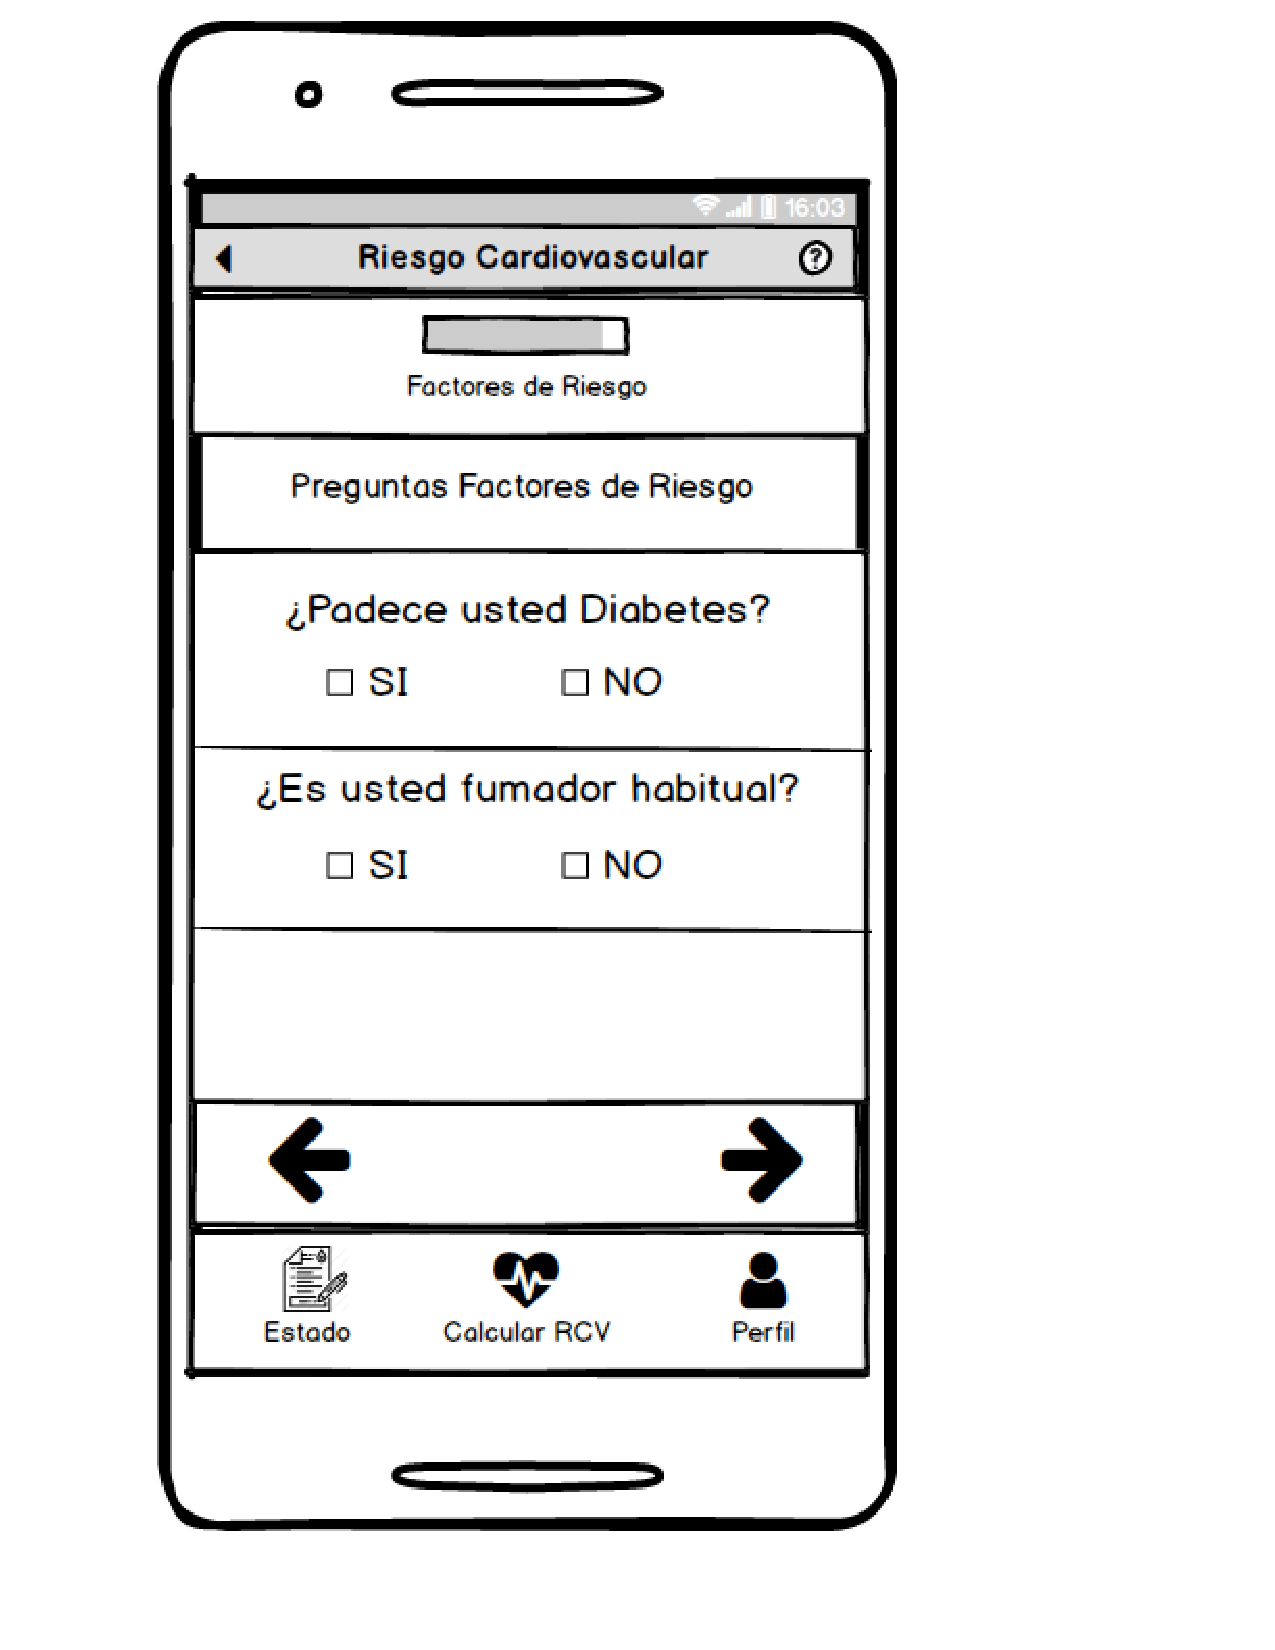
\includegraphics[width=0.3\textwidth]{GSI-9}
			\label{fig:raCalculo6}
		}
		\subfigure[]{
			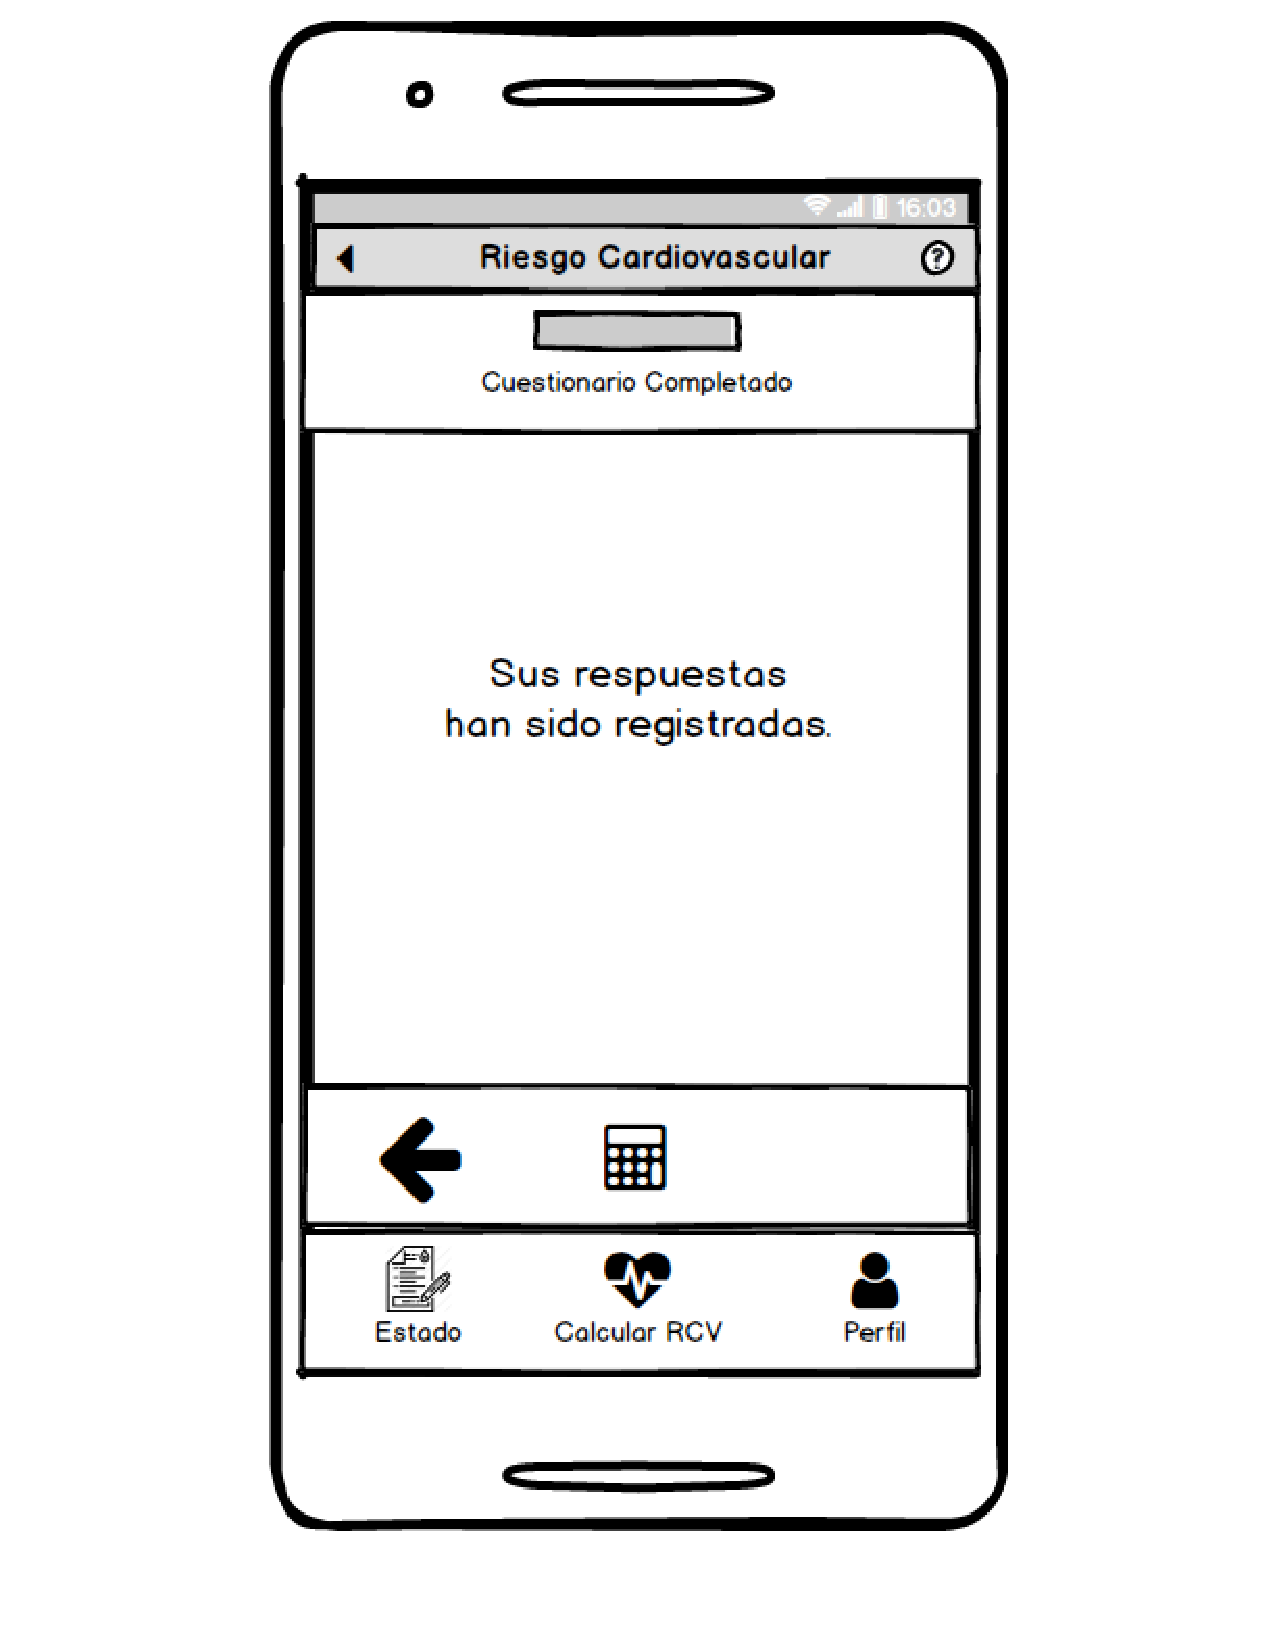
\includegraphics[width=0.3\textwidth]{GSI-10}
			\label{fig:raCalculo7}
		}
	\caption{Ventana Cálculo del RCV}
	\label{fig:cirugiaRA}
\end{figure}



\textbf{\textcolor{red}{\huge PENDIENTE}}